% \documentclass[tikz,convert=false,12pt]{standalone}

\documentclass[usletter,landscape]{article}
\usepackage{tikz}
\usepackage{color}
\usetikzlibrary{calc}
\usetikzlibrary{arrows}
\usetikzlibrary{shapes.geometric,positioning}




\renewcommand*\familydefault{\sfdefault} 
\renewcommand\familydefault{\sfdefault} 
\usepackage[T1]{fontenc}
\begin{document}
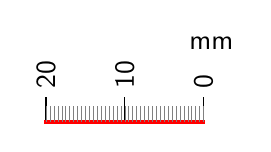
\begin{tikzpicture}[x=-1mm,line cap=rect]
  \foreach \i in {0,...,0}{ %i
    \tikzset{yshift=\i0mm}
    \node[color=black]  at (-1,1) {mm};
    \foreach \x in {0,10,...,20}  % x
    \draw [color=black, line width=0.20 mm, ](\x,0mm) -- (\x,3.0mm)
    node [color=black, rotate=90, anchor=west] {\pgfmathprint{int(\x+\i*100)}};
    
    %% horizontal line
    \draw [draw=red, line width=0.5 mm](0, 0mm) -- coordinate (x axis mid) (20,0mm);
    \foreach \x in {0,0.5,...,20}  % x
    \draw[color=gray, line width=0.05mm](\x,0mm) -- (\x, 2.0mm){};

}
\end{tikzpicture}

% \begin{tikzpicture}[x=-1cm,line cap=rect]
%   \foreach \i in {0,...,0}{ %i
%     \tikzset{yshift=\i0mm}
%     \node[color=black]  at (-1,1) {cm};
%     \foreach \x in {0,1,...,5}  % x
%     \draw [color=black, line width=0.10 cm, ](\x,0cm) -- (\x,0.8cm)
%     node [color=black, rotate=90, anchor=west] {\pgfmathprint{int(\x+\i*100)}};
    
%     %% horizontal line
%     \draw [draw=red, line width=0.1 cm](0, 0cm) -- coordinate (x axis mid) (5,0cm);
%     \foreach \x in {0,0.5,...,5}  % x
%     \draw[color=gray, line width=0.05cm](\x,0cm) -- (\x, 0.4cm){};

% }
% \end{tikzpicture}


\end{document}